\chapter{Introducción}
\label{cap:capitulo1}
\setcounter{page}{1}

En la actualidad, la tecnología forma parte de nuestro día a día. Prácticamente, constituye un elemento imprescindible para llevar a cabo cualquier actividad, sea profesional o cotidiana. Su función consiste en solucionar problemas para hacernos la vida más sencilla.\\

Con esto en mente, se presenta la \textbf{robótica} que, según la \ac{RAE}, se define cómo \emph{``técnica que aplica la informática al diseño y empleo de aparatos que, en sustitución de personas, realizan operaciones o trabajos, por lo general en instalaciones industriales.''} (Real Academia Española, s.f., definición 2) \footnote[1]{\href{https://dle.rae.es/rob\%C3\%B3tico\#WYTncqf}{https://dle.rae.es/robótico\#WYTncqf}}. Sin embargo, no es precisa, por ello una definición más concreta podría ser, ciencia que engloba diversas ramas tecnológicas, encargada del estudio y diseño de dispositivos mecánicos, provistos de sensores y actuadores, capaces de realizar tareas a través de la extracción y posterior procesamiento de la información, con el fin de generar respuestas adecuadas para resolver determinados problemas \footnote[2]{\url{https://revistaderobots.com/robots-y-robotica/que-es-la-robotica/?cn-reloaded=1}}.\\

Dentro de la robótica, existen diversas maneras de clasificar, sin embargo, una de las más comunes esta relacionada con la movilidad del dispositivo, esto es, si el mecanismo se puede desplazar por su entorno o no, por tanto se distingue lo siguiente:

\begin{enumerate}
	\item \textbf{Robótica industrial}: que involucra mecanismos fijos, capaces de realizar tareas de manera rápida, precisa y eficiente. Como es el caso de los brazos robóticos \footnote[3]{\url{https://www.geeksforgeeks.org/industrial-robots/}}.

	\item \textbf{Robótica móvil}: la cual abarca a los dispositivos móviles que se engloban en múltiples entornos y aplicaciones, como pueden ser, robótica aérea, terrestre y submarina \footnote[4]{\url{https://www.geeksforgeeks.org/mobile-robots/}}.
\end{enumerate}

\begin{figure} [h]
	\centering
	\subfigure[Robot industrial ABB]{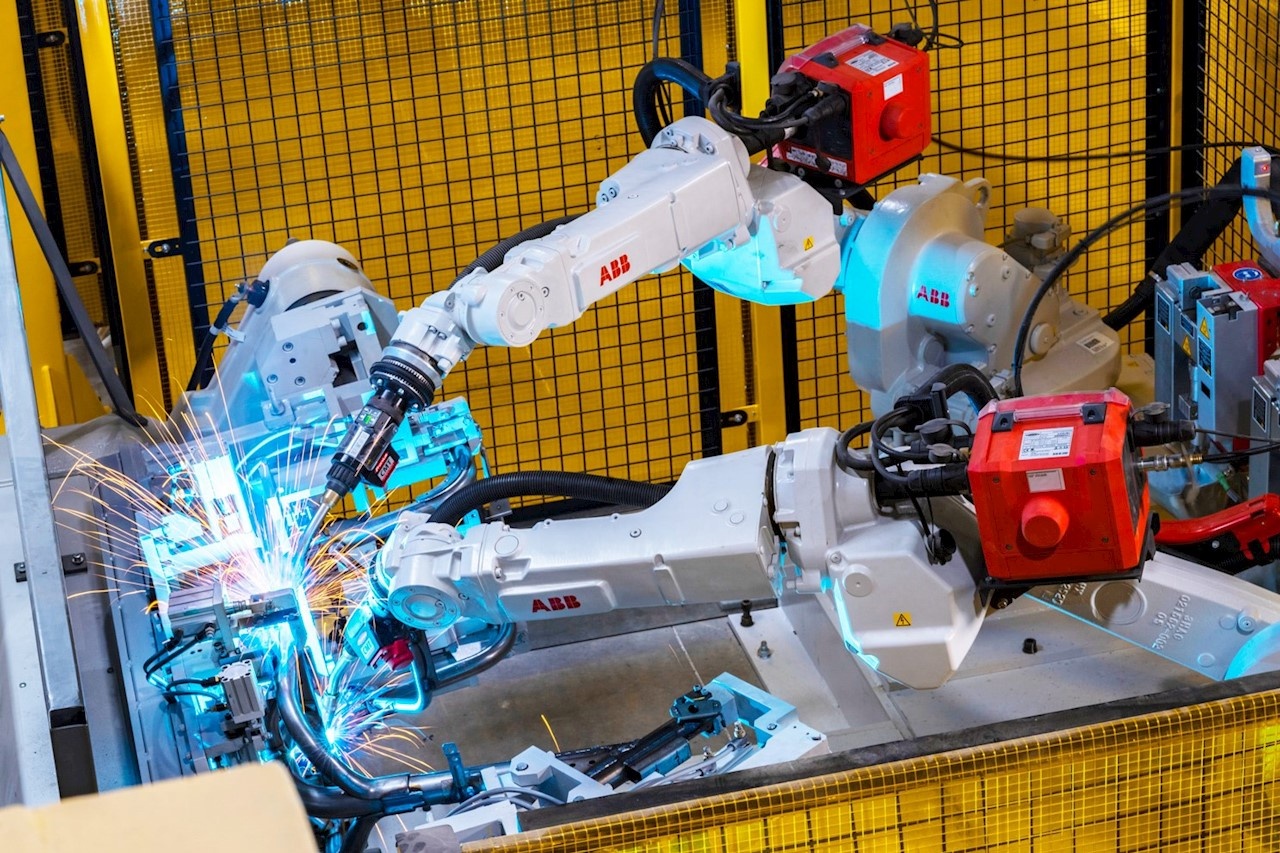
\includegraphics[height=3cm]{imagenes/cap1/1_industrial_robot.jpeg}}
	\quad
	\subfigure[Robot móvil Spot]{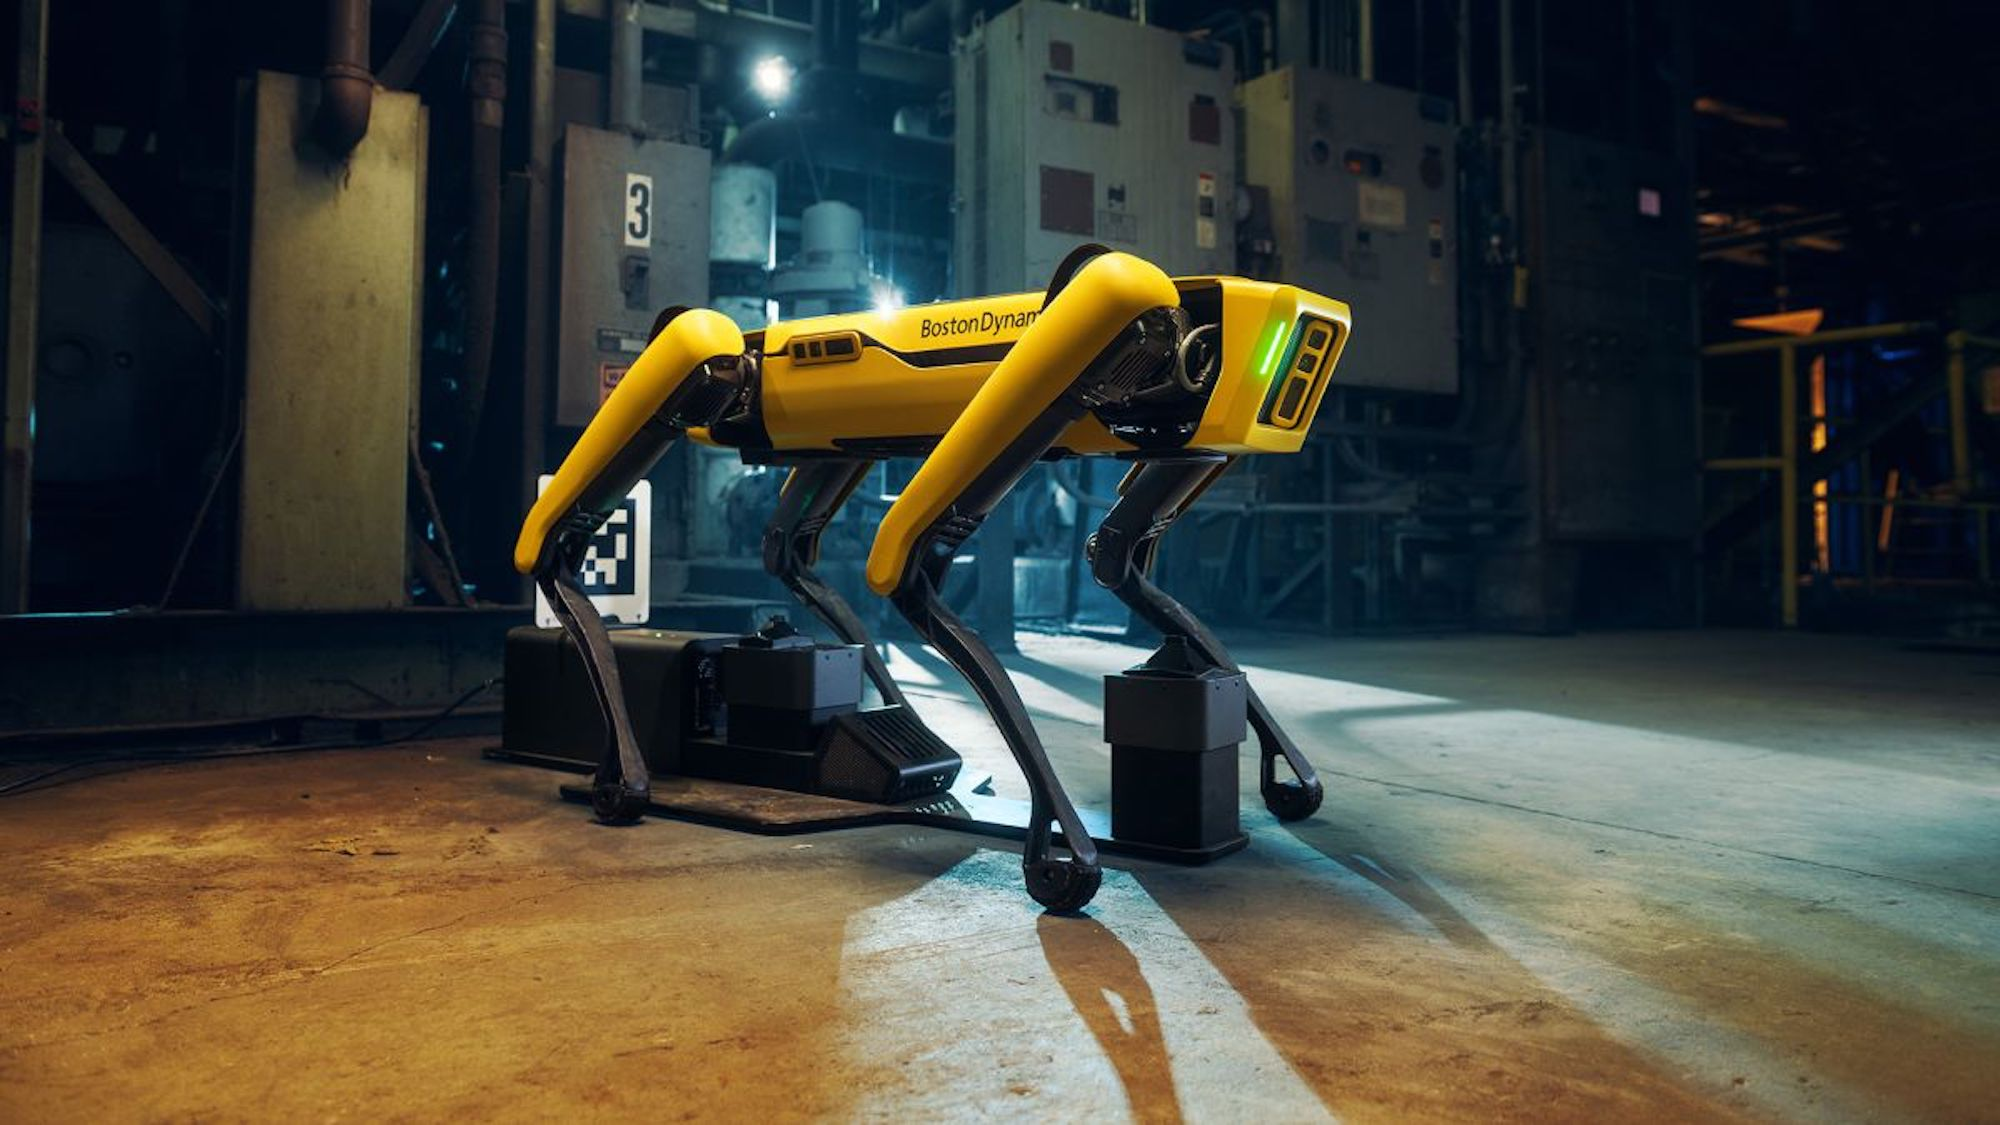
\includegraphics[height=3cm]{imagenes/cap1/2_mobile_robot.jpeg}}
	\quad
	\subfigure[Robot móvil aéreo]{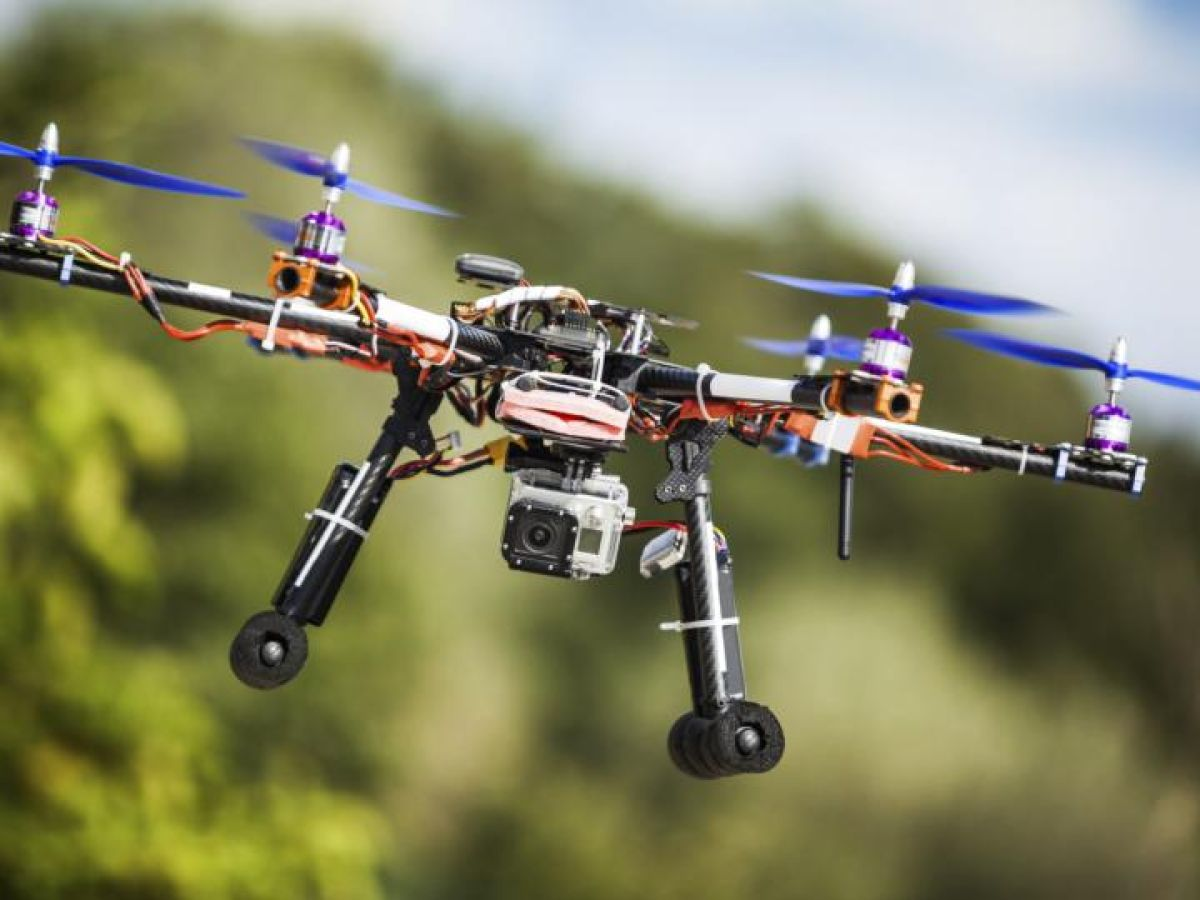
\includegraphics[height=3cm]{imagenes/cap1/1-5_real_drone.jpeg}}
	\caption{Robótica industrial VS robótica móvil}
	\label{fig:industrial_vs_mobile}
\end{figure}

Como tal, la robótica ayuda a resolver tareas repetitivas, peligrosas, delicadas y en ambientes problemáticos (conocidas como las 4 D's, \emph{dull, dirty, dangerous and dear}) \footnote[5]{\url{https://bernardmarr.com/the-4-ds-of-robotisation-dull-dirty-dangerous-and-dear/}}. Sin embargo, uno de los problemas más complicados de abordar, es el \textbf{contexto}, es decir, la capacidad de entender y adaptarse a las circunstancias del problema, como por ejemplo en el caso de la conducción autónoma, donde detectar un simple peatón, puede derivar en infinitos inconvenientes (condiciones de visibilidad, clima, atuendo, entre muchos otros). Es ahí, donde se presenta el segundo punto importante, la \ac{IA} \cite{dworakowski2020robots}.\\

\section{Robots}
\label{sec:robots}

Un robot es un dispositivo provisto con \textbf{sensores}, o elementos capaces de extraer información del entorno (por ejemplo una cámara), \textbf{actuadores}, o elementos que permiten al dispositivo realizar acciones (por ejemplo un motor), y una \textbf{unidad de procesamiento}, que se encarga de generar acciones a través de la información obtenida con los sensores, todo ello mediante algoritmos \cite{Wang2022}.\\

\begin{figure} [H]
	\begin{center}
	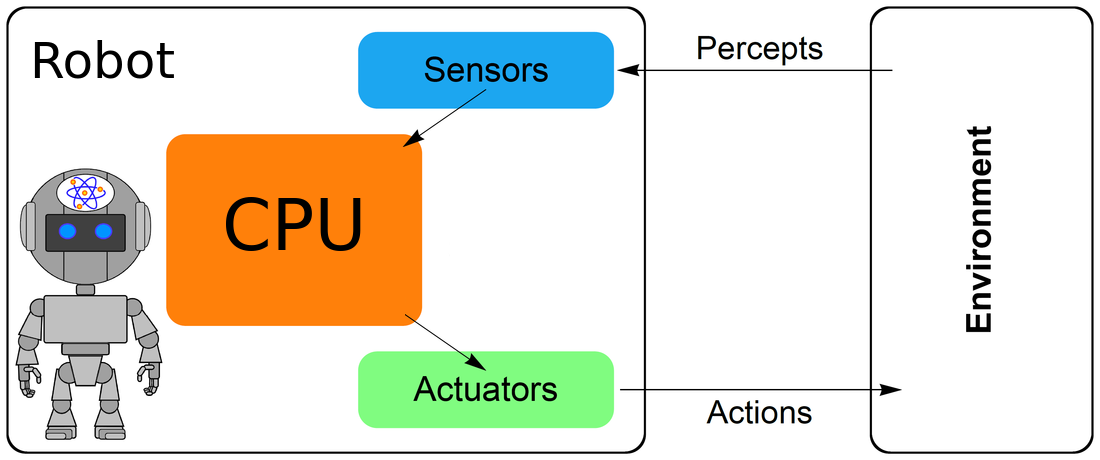
\includegraphics[height=5cm]{imagenes/cap1/3_robot.png}
	\end{center}
	\caption[Definición de robot]{Definición de robot}
	\label{fig:robot_def}
\end{figure}

Según el problema que se quiera resolver conviene usar unos u otros. En nuestro caso buscamos un robot con capacidad de navegar, preferiblemente grandes distancias y que pueda tomar medidas de la intensidad de una señal de forma autónoma.\\

Existen múltiples robots capaces de satisfacer estas condiciones, vease, los \ac{AGV}/\ac{AMR} o plataformas robóticas terrestres ampliamente empleadas logística, que permiten mover mercancía y navegar de forma autónoma por almacenes y naves industriales \footnote[6]{\url{https://www.mobile-industrial-robots.com/insights/get-started-with-amrs/agv-vs-amr-whats-the-difference/}}; los robots bipedos, los cuales emulan el movimiento humanoide, lo que aumenta su adaptabilidad a cualquier entorno real (ya que el mundo esta diseñado para la biomecánica humana), sin embargo, son bastante complejos debido a la dificultad de replicar la marcha bípeda \cite{10.3389/fmech.2020.00011}; y por último, los drones, empleados en labores de \ac{SAR}, o de inspección en lugares poco accesibles, entre otros.

\subsection{Drones}
\label{subsec:drones}

Los \ac{UAS} tienen origen en la primera guerra mundial, con el biplano llamado \textbf{Kettering bug}. Se trataba de un torpedo que era lanzado desde una carretilla, capaz de volar de forma no tripulada, hasta que se liberaba de sus alas y caía sobre el objetivo \footnote[7]{\url{https://www.nationalmuseum.af.mil/Visit/Museum-Exhibits/Fact-Sheets/Display/Article/198095/kettering-aerial-torpedo-bug/}}. Más tarde, entre la primera y segunda guerra mundial (1935), se diseño el \textbf{Queen Bee}, de donde surgió el termino \emph{``drone''}, como abeja macho en busca de la reina, que se trataba de un avión no tripulado, con el fin de servir de objetivo para realizar prácticas de artillería aérea \footnote[8]{\url{https://www.dehavillandmuseum.co.uk/aircraft/de-havilland-dh82b-queen-bee/}}. Sin embargo, no fue hasta \textbf{Operation Aphrodite}, en la segunda guerra mundial, donde realmente se vió el primer dron radio tripulado, con el fin de poder volar en entornos ``sucios'' o dirty, dado el nuevo paradigma de las bombas atómicas \footnote[9]{\url{https://warfarehistorynetwork.com/article/operation-aphrodite/}}.\\

\begin{figure} [h]
	\centering
	\subfigure[Kettering Bug]{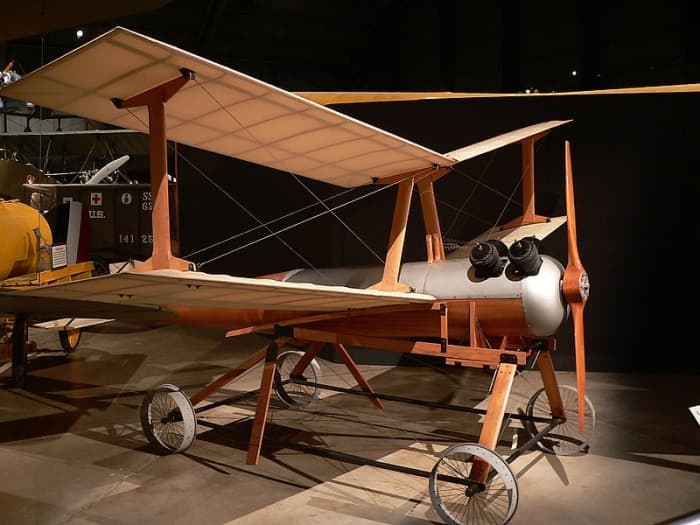
\includegraphics[height=2.5cm]{imagenes/cap1/4_kettering_bug.jpeg}}
	\quad
	\subfigure[Queen Bee]{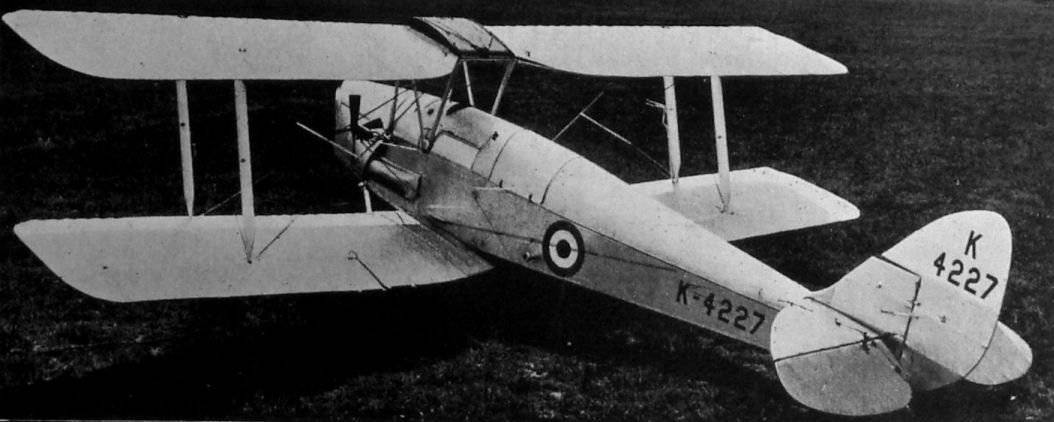
\includegraphics[height=2.5cm]{imagenes/cap1/5_queen_bee.jpeg}}
	\quad
	\subfigure[Aphrodite Operation]{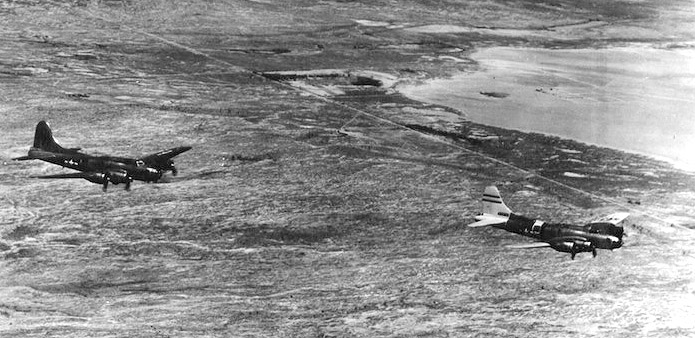
\includegraphics[height=2.5cm]{imagenes/cap1/6_aphrodite.jpeg}}
	\caption{Historia de los drones}
	\label{fig:drone_history}
\end{figure}

Existen múltiples avances y ejemplos posteriores, pero en la actualidad podemos definir un \textbf{\ac{UAS}} teniendo en cuenta lo siguiente:

\begin{enumerate}
	\item \textbf{\ac{GCS}}: es la estación de tierra o el elemento encargado de controlar la nave \footnote[10]{\url{https://www.trentonsystems.com/blog/ground-control-stations}}

	\item \textbf{Comunicación}: conecta y gestiona la transmisión de datos entre el \ac{UAV} y la \ac{GCS}, mediante \textbf{data links}, o canales de transmisión \cite{data-link-definicion}.
	
    \item \textbf{\ac{UAV}}: hace referencia directamente a la aeronave.
\end{enumerate} \footnote[11]{\url{https://srmconsulting.es/blog/uav-uas-rpa-dron-como-llamarlos.html}}

\begin{figure} [H]
	\begin{center}
	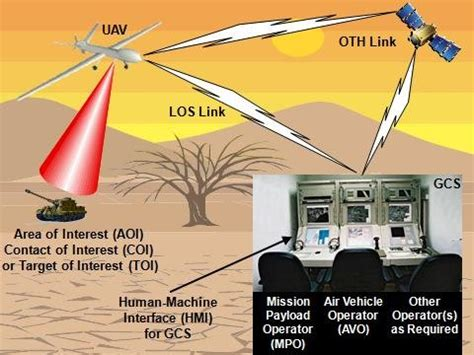
\includegraphics[height=6cm]{imagenes/cap1/7_drone_components.jpeg}
	\end{center}
	\caption[Descripción gráfica de \ac{UAS} (GCS + Data Links + UAV)]{Descripción gráfica de \ac{UAS} (GCS + Data Links + UAV)}
	\label{fig:drone_components}
\end{figure}

También cabe destacar que hay variedad de drones, según su peso y capacidad de carga de pago, o elementos que sea capaz de cargar, lo cual influye en la \textbf{legislación} detras de su uso (de forma general, cuanto mayor sea el peso, más legislación debe cumplir y mayores restricciones de uso tiene) \footnote[12]{\url{https://www.safedroneflying.aero/en/drone-guide/drone-regulations}}.\\

Tal y como fue mencionado, la gran ventaja del uso de vehículos aéreos es poder evitar las irregularidades del terreno, sin embargo, hay ligados al uso de estos dispositivos ciertos problemas, como son el clima, la carga de pago que afecta a la autonomía (peso de las baterías), los interiores (afectan a la señal GPS), entre otros.\\

Agrupando la robótica y los drones, se pueden observar múltiples ejemplos de uso, uno muy conocido es el de un dron \emph{``sigue-persona''}, el cual permite a un \ac{SUAV} detectar y moverse al son de un objetivo móvil, tal y como puede ser una persona; o bien para controlar desastres naturales, como por ejemplo un incendio, donde mediante visión artificial se puedan localizar y controlar los focos activos \footnote[13]{https://www.euronews.com/2023/09/19/could-ai-powered-drones-be-the-solution-to-europes-wildfire-problems}.

\section{Inteligencia artificial}
\label{subsec:inteligencia_artificial}

% La \ac{IA} ha tenido un auge importante en los últimos años, especialmente en el ámbito de la robótica dado su amplio abanico de soluciones sinérgicas con la misma, sin embargo, conviene conocer lo origenes. Quizás, la primera pregunta que se buscó responder fue la siguiente \textbf{¿Puede una máquina pensar?}, formulada en \emph{``Computing Machinery and Intelligence''} (Alan Turing, 1950), de donde surgió el famoso test de Turing, entre otras ideas \cite{turing-paper}. La búsqueda de la \ac{IA} enfrentó desafíos iniciales debido a la incapacidad de las primeras computadoras para almacenar datos y su elevado precio. Sin embargo, en 1956, se presentó el primer programa de \ac{IA} llamado \textbf{Logic Theorist} en el \textbf{Dartmouth Summer Research Project on Artificial Intelligence} \cite{logic-theorist}. Con el tiempo, la IA progresó con mejores algoritmos y mejoras en la capacidad de las computadoras. A pesar de esto, lograr los objetivos finales de la IA, como comprender el lenguaje humano y el pensamiento abstracto, sigue siendo un desafío a día de hoy \cite{history-ai}.\\

La \ac{IA} ha tenido un auge importante en los últimos años, especialmente en el ámbito de la robótica dado su amplio abanico de soluciones sinérgicas con la misma, desde \emph{``Computing Machinery and Intelligence''} (Alan Turing, 1950), donde se buscó responder fue la siguiente \textbf{¿Puede una máquina pensar?}, formulada en \emph{``Computing Machinery and Intelligence''} (Alan Turing, 1950); pasando por \textbf{Logic Theorist} en el \textbf{Dartmouth Summer Research Project on Artificial Intelligence} \cite{logic-theorist}; hasta la actualidad, donde los algoritmos mejoraron a la par de la capacidad de computación, destacando por ejemplo la navegación autónoma, empleada en drones entre otros vehículos \footnote[14]{\url{https://sitn.hms.harvard.edu/flash/2017/history-artificial-intelligence/}}.\\

En general, la \ac{IA} es capaz de abordar los siguientes problemas de aprendizaje:

\begin{enumerate}
	\item \textbf{Supervisado}: es decir, se emplea un conjunto de datos del que se conocen tanto las salidas cómo las entradas a las que pertenecen. La idea es conseguir obtener una salida precisa dada una entrada concreta. Por ejemplo, dados los metros cuadrados de una vivienda (entrada), obtener su precio estimado (salida).

	\item \textbf{No supervisado}: donde se tiene un conjunto de datos de entrada de los que no se conoce la salida. Básicamente, se encarga de distribuir dicho conjunto en sets con características comunes. Un ejemplo común es la segmentación de imagenes, donde se clasifica cada elemento de la imagen según su naturaleza.
	
    \item \textbf{Por refuerzo}: resuelve un problema a base de prueba y error, mediante un sistema de recompensas. Como por ejemplo \emph{``Stockfish''}, que es un modelo entrenado para ganar una partida de ajedrez en el menor número de movimientos posible, superando incluso a grandes maestros de la actualidad \footnote[15]{\url{https://stockfishchess.org/about/}}.
\end{enumerate} \footnote[16]{\url{https://www.springboard.com/blog/data-science/regression-vs-classification/}}

\begin{figure} [H]
	\begin{center}
	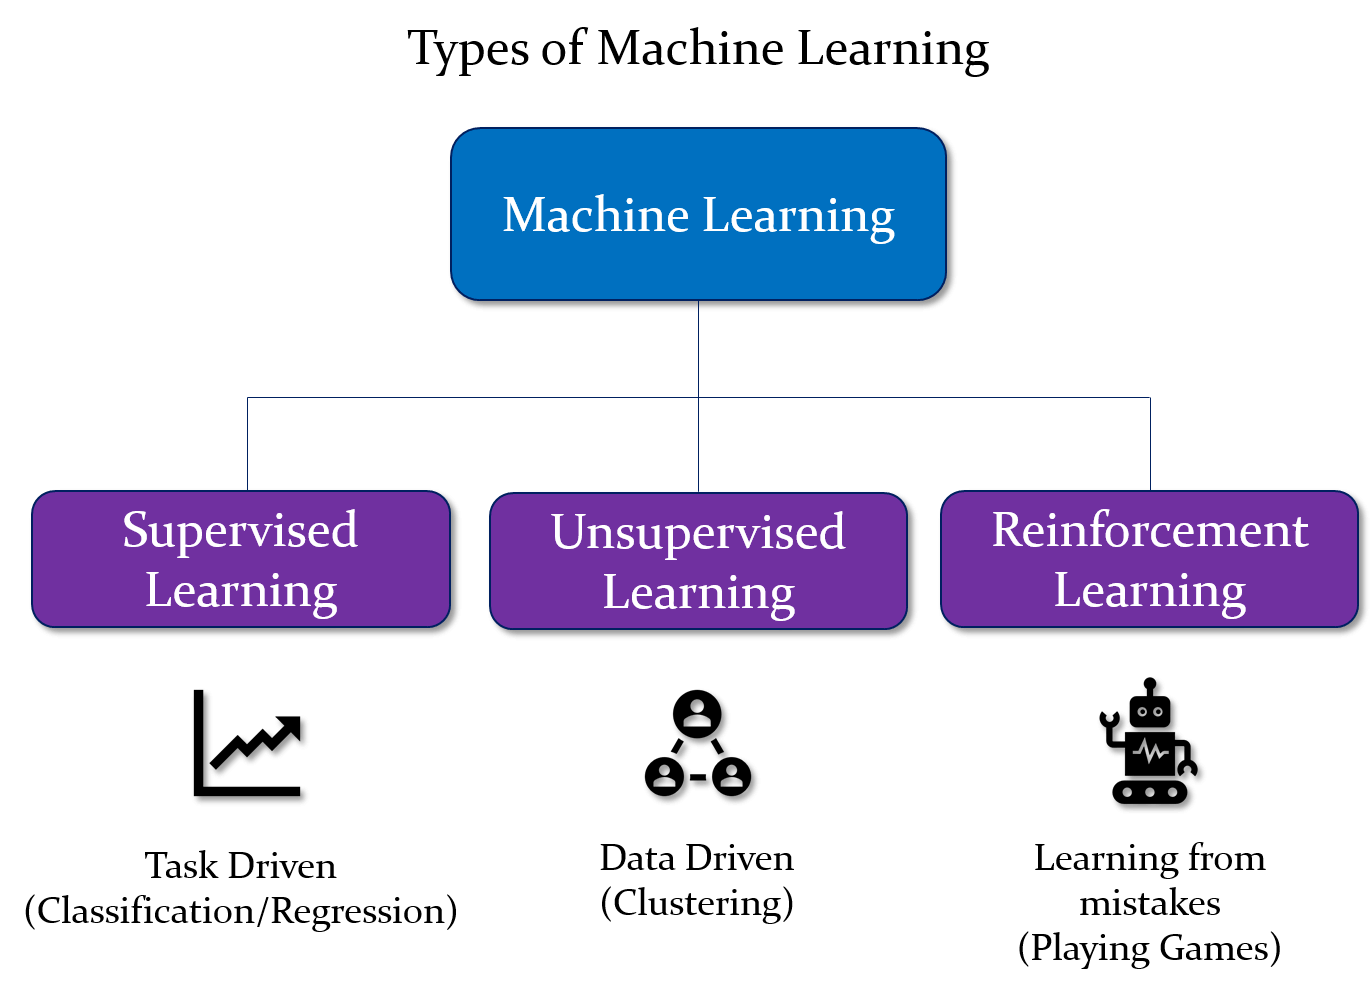
\includegraphics[height=5.5cm]{imagenes/cap1/8_AI_types.png}
	\end{center}
	\caption[Clasificación de aprendizaje máquina]{Clasificación de aprendizaje máquina}
	\label{fig:ai_types}
\end{figure}

\subsection{Aprendizaje por refuerzo}
\label{subsec:aprendizaje_por_refuerzo}

Se basa en un sistema de \textbf{recompensas y penalizaciones}, que permite entrenar a un modelo para converger hacia la toma de buenas decisiones. Este enfoque se basa en los llamados \textbf{procesos de Markov}, que se definen como aquellos que, para un instante dado, contienen toda la información relevante sin depender de todos los procesos anteriores. \footnote[17]{\url{https://www.geeksforgeeks.org/what-is-reinforcement-learning/}}\\

En particular, hablamos de \textbf{agente}, o modelo encargado de tomar decisiones en un \textbf{entorno} (que es el medio en el que interactúa dicho agente, y está regido por una serie de reglas); \textbf{estados}, o circunstancias en la que se sitúa el agente en un determinado instante temporal; y \textbf{acciones}, o decisiones que toma el agente y que le permiten cambiar de estado. En términos de Markov, decimos que el estado actual no depende de todos los estados previos. \footnote[18]{\url{https://www.alexanderthamm.com/es/blog/refuerzo-aprendizaje-marco-y-ejemplo-de-aplicacion/}}\\

\begin{figure} [H]
	\begin{center}
	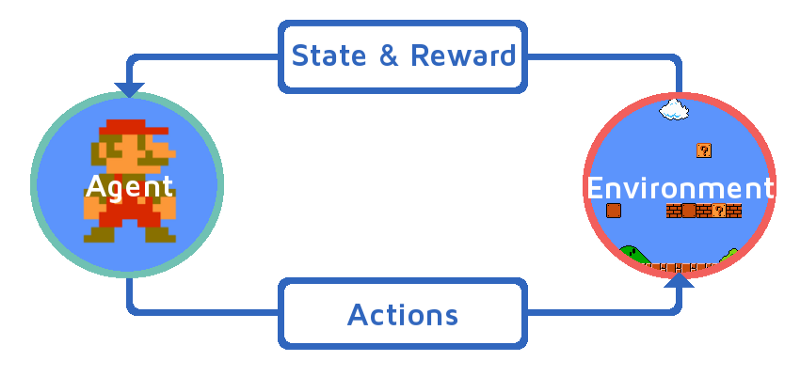
\includegraphics[height=4cm]{imagenes/cap1/9_reinforcement.png}
	\end{center}
	\caption[Aprendizaje por refuerzo]{Aprendizaje por refuerzo}
	\label{fig:reinforcement_learning}
\end{figure}

Cabe destacar que, este enfoque está directamente extraido de la \textbf{psicología} y el estudio del comportamiento, donde en función de recompensas y castigos se induce al aprendizaje en distintas tareas, como por ejemplo, enseñar a jugar al ping pong a dos palomas \footnote[19]{\url{https://pressbooks.online.ucf.edu/lumenpsychology/chapter/operant-conditioning/} \url{https://pressbooks-dev.oer.hawaii.edu/psychology/chapter/operant-conditioning/}}.\\

Entre los distintos modelos, encontramos \textbf{Q-Learning}, que busca generar una tabla numérica donde cada fila se interprete como un estado del robot, que puede ser su posición; y cada columna sea una determinada acción, como puede ser moverse hacia algún lugar. De este modo, y a través de una \textbf{función de recompensa}, se rellenan los valores de la tabla, los cuales, según el tipo de función escogida, convergerá comportamientos de un tipo u otro. Una vez obtenida la tabla, el robot solo debe identificar en que estado se encuentra (fila) y elegir la columna con mayor valor numérico, lo que se traducirá en la mejor acción para dicho estado \footnote[20]{\url{https://towardsdatascience.com/reinforcement-learning-explained-visually-part-4-q-learning-step-by-step-b65efb731d3e}}.\\

Existen múltiples ejemplos de aplicación de esta metodología a casos reales, vease para controlar de forma adaptativa una señal de tráfico; para jugar a la Atari 2600; o para realizar un control híbrido sobre la navegación de un robot, entre otros. \cite{q-learning-app}\\

\section{Vigilancia del espectro electromagnético}
\label{subsec:señales}

Las comunicaciones inalámbricas son aquellas donde tanto el emisor como el receptor se intercambian información sin el uso de cables u otros medios similares. En su defecto usan ondas electromagnéticas moduladas transmitidas generalmente por el aire. En este caso concreto, hablamos de señales \ac{RF}, como son por ejemplo Wi-Fi, radio FM, 4G, 5G, entre otros tipos de señales distribuidas a lo largo del espectro.\\

Dicho espectro se divide por bandas de frecuencia, que se reparten para diversos uso. El ejemplo más claro es la banda FM de radio, que se reparte entre los 87-108 MHz para España, donde cada emisora tiene un ancho asignado para emitir. \footnote[21]{\url{https://www.wikiwand.com/en/FM_broadcast_band}}\\

De este modo, se pueden encontrar soluciones a problemas como el rastreo de una señal de móvil para una persona perdida en la montaña, o seguir emisores concretos, como pueden ser convoys, o también en casos de ataques del tipo jamming (introducción de interferencias para invalidar la comunicación), donde se necesite hallar el origen del ataque, entre otros. Lo único que hay que establecer, es la banda de frecuencia adecuada y establecer un comportamiento que permita navegar hasta la señal de manera autónoma.\\

\section{Síntesis}
\label{subsec:sintesis}

Este proyecto se centra en desarrollar un comportamiento autónomo de un dron, basado en aprendizaje por refuerzo, con el fin de identificar un transmisor \ac{RF} en un entorno dinámico, es decir, en el cual se sorteen obstáculos de camino al origen de la señal.

% Para finalizar, cabe destacar algunos proyectos relacionados, donde se puede ver el uso conjunto de drones y robótica para la creación de un módulo ROS, en el que se engloban las comunicaciones para programar un sigue-persona \cite{tfm-pedro}, junto con el uso de estas aeronaves en síntesis con la \ac{IA}, para lograr la navegación en interiores de la misma \cite{paper-ia-dron}\\

En nuestro caso, se usará un dron del tipo \ac{SUAV}, provisto de un receptor \ac{RF} como sensor. Se le agregarán algoritmos sistemáticos para compararlos con soluciones Q-Learning.